%% ============================================================================
%% §4.3.2 FPGA Backend  --  Zynq UltraScale+ bring-up
%% ============================================================================
\subsubsection{FPGA Backend: Vivado on Zynq UltraScale+}
\label{sec:hw:backend:fpga}

The same RTL is synthesised in Vivado and implemented on a Zynq UltraScale+ MPSoC. The Processing System (PS) hosts a Python control program that loads weights and image into the on-chip BRAMs, asserts a pulse-start signal to the NPU, waits for the done flag, and reads the 128-d embedding back over AXI. Figure~\ref{fig:fpga_block} shows the resulting block design: the PS-side ZYNQ UltraScale+ MPSoC block is connected to the NPU through an AXI Interconnect and three AXI-GPIO blocks (control signals, address bus, and 128-bit readout bus).

\begin{figure}[H]
  \centering
  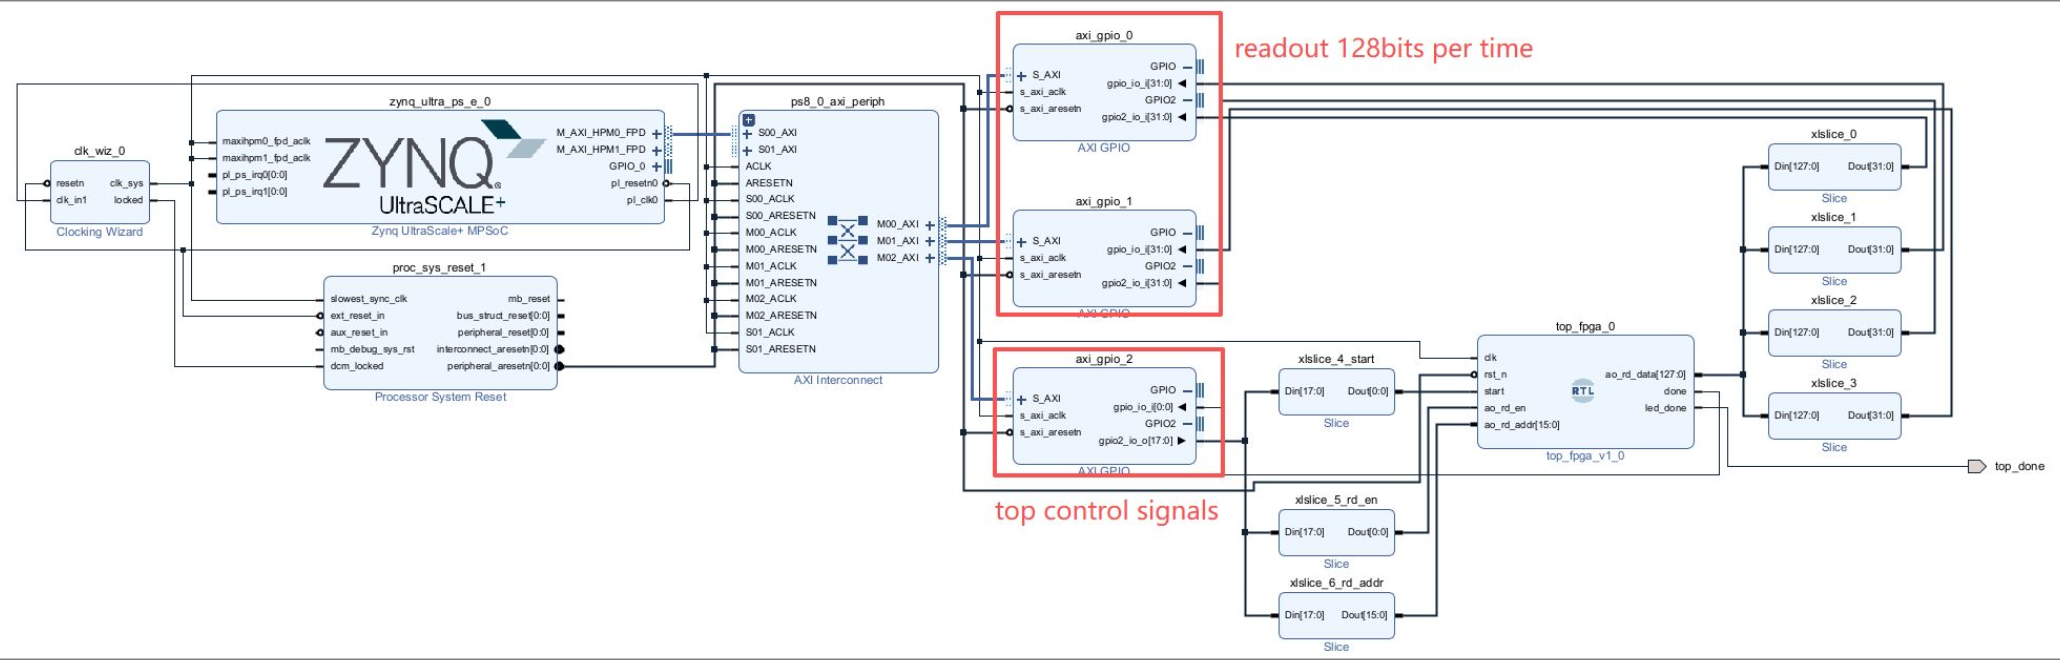
\includegraphics[width=0.95\textwidth]{Fig/peixing/fpga_backend.png}
  \caption[FPGA block design (Vivado IP integrator).]{FPGA block design. The PS triggers NPU execution via a control AXI-GPIO; the address bus drives the A/O RAM readout; the readout bus returns 128-bit words to the PS for embedding reconstruction.}
  \label{fig:fpga_block}
\end{figure}

\paragraph{Resource utilisation.}
Vivado implementation reports the resource usage in Table~\ref{tab:fpga_resource}. The BRAM utilisation is the dominant resource at 54\,\%, reflecting the WGT RAM + A/O RAM + Param RAM footprint, while the DSP slice count remains low because most MACs map to LUTs in the SA fabric.

\begin{table}[H]
\centering
\caption{FPGA Resource Utilisation (Vivado Implementation)}
\label{tab:fpga_resource}
\begin{tabular}{lrrr}
\toprule
\textbf{Resource} & \textbf{Utilisation} & \textbf{Available} & \textbf{Util.\,\%} \\
\midrule
LUT     & 107{,}569 & 425{,}280 & 25.29 \\
LUTRAM  & 1{,}308   & 213{,}600 & 0.61 \\
FF      & 166{,}393 & 850{,}560 & 19.56 \\
BRAM    & 583       & 1{,}080   & 53.98 \\
DSP     & 421       & 4{,}272   & 9.85 \\
IO      & 1         & 347       & 0.29 \\
BUFG    & 5         & 696       & 0.72 \\
MMCM    & 1         & 8         & 12.50 \\
\bottomrule
\end{tabular}
\end{table}

\paragraph{Performance.}
The bitstream meets timing at 150\,MHz and the NPU completes one $112\times96$ inference in 19{,}175{,}557 cycles, i.e.\ 127.8\,ms per image. Compared against a reference INT8 PyTorch run on an Intel i7-9700 at 3.0\,GHz (917.37\,ms per image), this is a $\times7.18$ speed-up (Table~\ref{tab:fpga_speedup}).

\begin{table}[H]
\centering
\caption{FPGA Throughput Comparison (one inference, $112\times96$ image)}
\label{tab:fpga_speedup}
\begin{tabular}{lcc}
\toprule
 & \textbf{NPU on Zynq} & \textbf{i7-9700 @ 3.0\,GHz} \\
\midrule
Frequency        & 150\,MHz       & 3.0\,GHz \\
Total cycles     & 19{,}175{,}557 & -- \\
Execution time   & 127.8\,ms      & 917.37\,ms \\
Speed-up         & $\times7.18$   & $\times1$ \\
\bottomrule
\end{tabular}
\end{table}

A faster RFSoC 4x2 part (PL fabric reaches 500\,MHz on the same NPU) would give an estimated $\times43.08$ speed-up over the same i7-9700 baseline; this remains future work.
